\documentclass[11pt]{article}

\usepackage[margin=1in]{geometry}
\usepackage{times}
\usepackage{booktabs}
\usepackage{array}
\usepackage{longtable}
\usepackage{xcolor}
\usepackage{enumitem}
\usepackage{hyperref}
\usepackage{graphicx}
\usepackage{amsmath}
\usepackage{amssymb}
\usepackage{tikz}
\usetikzlibrary{arrows.meta,positioning,fit,backgrounds}

\hypersetup{colorlinks=true,linkcolor=blue,citecolor=blue,urlcolor=blue}
\sloppy
\emergencystretch=3em

\newcommand{\status}[1]{%
  \ifx#1P\textcolor{blue!60!black}{\textbf{Present}}\fi
  \ifx#1A\textcolor{orange!80!black}{\textbf{Partial}}\fi
  \ifx#1M\textcolor{red!70!black}{\textbf{Missing}}\fi
}

\title{Integration Plan:\\From a Pretrained LiDAR 3D Detector to a\\DSP-SLAM++-Style Multi-Class Object SLAM Pipeline}
\author{Planning document for \texttt{Code\_tensor}}
\date{\today}

\begin{document}
\maketitle

\begin{abstract}
This document plans the work required to grow the existing \texttt{lidar\_detection} module --- a trained PointPillars backbone with a CenterPoint detection head \cite{yin2021center}, using the \texttt{checkpoint\_nuscenes\_center.pth} weights --- into a full object-aware SLAM system that reproduces the architecture of DSP-SLAM++ \cite{kourani2026dspslampp}, itself an extension of DSP-SLAM \cite{wang2021dspslam}. It inventories what the current repository already provides, maps every remaining paper component to a concrete work package, sequences those work packages by dependency, and flags the architectural decisions and risks that should be resolved before implementation starts. No source code is modified by this document; it is a planning artifact only.
\end{abstract}

\tableofcontents

% ----------------------------------------------------------------------
\section{Scope and Starting Point}

The repository currently implements one block of the target system: the \emph{3D detection candidate generator} (``Det3D'' in Algorithm 1, line 2, of \cite{kourani2026dspslampp}). Concretely:

\begin{itemize}[nosep]
  \item \texttt{lidar\_detection/models/pointpillars.py} --- PointPillars \cite{lang2019pointpillars} backbone; both an anchor head (\texttt{PointPillars}) and a CenterPoint heatmap head \cite{yin2021center} (\texttt{CenterPointPillars}) are implemented. \textbf{This plan standardizes on the CenterPoint head}, per the project decision to use \texttt{checkpoint\_nuscenes\_center.pth}.
  \item \texttt{lidar\_detection/detection/center\_postprocess.py} --- heatmap peak extraction (3$\times$3 max-pool NMS, top-$K$ per class) and box decoding for the CenterPoint head; this is the post-processing path relevant to this plan (the anchor-head path in \texttt{postprocess.py}/\texttt{anchor.py}/\texttt{nms.py} is not used going forward).
  \item \texttt{lidar\_detection/pipeline.py} --- \texttt{DetectionPipeline.run(points)} returns class-labeled 3D boxes \texttt{[x,y,z,l,w,h,yaw]} with scores, i.e. exactly the $d_{3D,i}$ tuples Algorithm~1 needs. \textbf{Note:} as currently written, \texttt{DetectionPipeline} hard-codes the anchor-head \texttt{PointPillars} model and the \texttt{postprocess} path; it does not yet know how to load \texttt{CenterPointPillars} or call \texttt{center\_postprocess}. Wiring \texttt{DetectionPipeline} to the CenterPoint head/checkpoint is therefore the first concrete change needed and is captured as part of WP1 (Section~\ref{sec:wps}).
  \item \texttt{lidar\_detection/data/nuscenes\_loader.py}, \texttt{train\_nuscenes.py}, \texttt{validate\_nuscenes.py} --- nuScenes \cite{caesar2020nuscenes} training/validation, reporting AP/mATE/mASE/mAOE/NDS; \texttt{train\_nuscenes.py --center} / \texttt{validate\_nuscenes.py --center} already select the CenterPoint path.
  \item Trained checkpoint \texttt{checkpoint\_nuscenes\_center.pth} (CenterPoint head) for classes \texttt{Car, Pedestrian, Cyclist}. (\texttt{checkpoint\_nuscenes.pth}, the anchor-head checkpoint, is superseded by this decision and is not part of the go-forward plan.)
\end{itemize}

Everything else in Fig.~2 of \cite{kourani2026dspslampp} --- the tracking thread, the 2D detector, the fisheye/LiDAR fusion, the association logic, the shape reconstruction back-end, the asynchronous pipeline, and the joint optimizer --- does not exist yet in this repository. The goal of this plan is to define, in order, what needs to be built to close that gap.

% ----------------------------------------------------------------------
\section{Gap Analysis}

Table~\ref{tab:gap} maps every architectural component of DSP-SLAM++ to its status in \texttt{Code\_tensor} today.

\begin{longtable}{p{4.1cm}p{1.6cm}p{1.5cm}p{6.3cm}}
\toprule
\textbf{Paper component} & \textbf{Paper ref.} & \textbf{Status} & \textbf{Notes} \\
\midrule
\endhead
3D object detection (PointPillars + CenterPoint head) & Sec.~IV-A & \status{P} & Present (\texttt{checkpoint\_nuscenes\_center.pth}), but (i) class set (\texttt{Car/Pedestrian/Cyclist}) does not match the target classes \texttt{car/bus/motorcycle/pedestrian}; (ii) per-class confidence thresholds $\tau_{c,3D}$ are not yet exposed per class in \texttt{center\_postprocess.py}; (iii) \texttt{DetectionPipeline} (\texttt{pipeline.py}) currently instantiates the anchor-head model only and must be extended to load \texttt{CenterPointPillars} and call \texttt{center\_postprocess}. \\
2D multi-class detection (YOLO11x-seg) & Sec.~IV-A, VII-A & \status{M} & No 2D detector, no instance segmentation masks, no class labels for the image stream. \\
Global greedy 2D--3D bipartite association & Sec.~IV-A, Eqs.~1--3 & \status{M} & Score matrix $S$, class-consistency gating, iterative arg-max assignment (Algorithm~1, lines 2--3) all absent. \\
Fisheye mask rectification & Sec.~VI, VII-E & \status{M} & Contour-based rectification of predicted masks before projection scoring; absent. \\
Class-aware map association (radius $r_c$) & Sec.~IV-B & \status{M} & Per-class matching radius from footprint diagonal, plus the second global re-association pass for loop closure/reappearance; absent. \\
Modular multi-decoder DeepSDF reconstruction & Sec.~IV-C & \status{M} & No DeepSDF decoders, no per-class latent code optimization, no pose $T_{co}$/shape $z_c$ refinement. \\
Asynchronous reconstruction back-end & Sec.~V, Algorithm~2 & \status{M} & Thread pool, task queue, result queue, bounding-box placeholder objects; absent. \\
Visual (fisheye) tracking front-end & Sec.~III, VI & \status{M} & No ORB-SLAM3 \cite{campos2021orbslam3} integration, no Kannala--Brandt \cite{kannala2006generic} camera model, no keyframe/tracking thread. \\
RGB-L metric depth fusion & Sec.~VI & \status{M} & LiDAR-to-feature depth association (feature-rectification strategy of \cite{sauerbeck2022rgbl}) absent; monocular scale ambiguity unresolved. \\
Joint map--object pose graph optimization & Sec.~III & \status{M} & Camera poses, sparse map points, and object pose/shape jointly refined at each keyframe; absent. \\
Streaming dataset adapters (synced image+LiDAR+pose, calibration) & Sec.~VII-A & \status{A} & \texttt{nuscenes\_loader.py} exists but is a training-time loader (batched, shuffled); a time-synchronized, per-frame streaming loader with calibration/extrinsics for SLAM playback is absent, as are KITTI and custom fisheye-LiDAR adapters. \\
Evaluation harness (ATE, latency tables) & Sec.~VII-B, D & \status{M} & No ATE trans/rot computation, no per-stage latency instrumentation (Detect./Object/Max Obj./KF~BA latency). \\
Visualization (3D object map + trajectory) & Sec.~VII-C, Fig.~7,9 & \status{A} & \texttt{lidar\_detection/visualization/visualizer.py} does BEV-only plots; 3D mesh map + trajectory overlay is absent. \\
\bottomrule
\caption{Component-by-component gap analysis against DSP-SLAM++.}
\label{tab:gap}
\end{longtable}

% ----------------------------------------------------------------------
\section{Target Architecture}

Figure~\ref{fig:arch} restates the DSP-SLAM++ thread architecture (Fig.~2 of \cite{kourani2026dspslampp}) and marks where the existing PointPillars pipeline plugs in versus what must be newly built.

\begin{figure}[h]
\centering
\resizebox{\textwidth}{!}{%
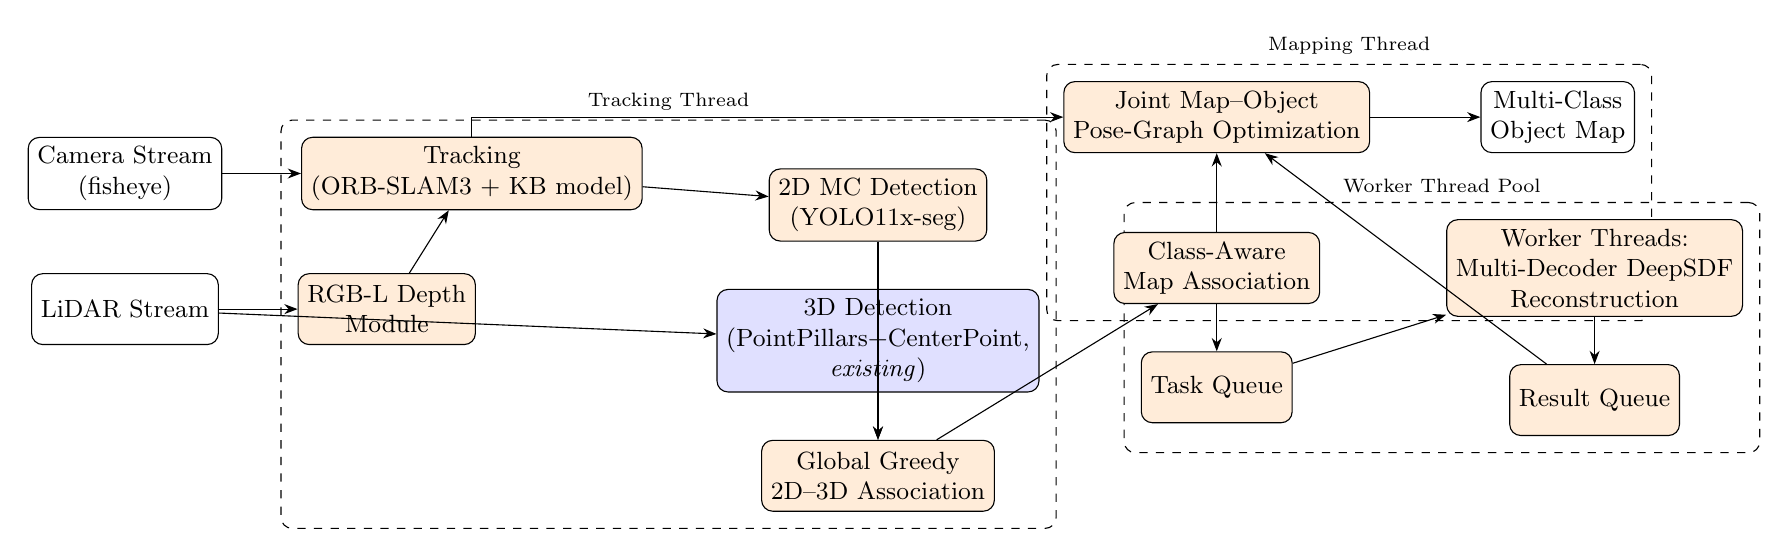
\begin{tikzpicture}[
  node distance=8mm and 10mm,
  block/.style={rectangle, draw, rounded corners, align=center, minimum height=9mm, font=\small},
  existing/.style={block, fill=blue!12},
  new/.style={block, fill=orange!15},
  thread/.style={draw, dashed, inner sep=6pt, rounded corners},
  >=Stealth
]

\node[block] (cam) {Camera Stream\\(fisheye)};
\node[block, below=of cam] (lidar) {LiDAR Stream};

\node[new, right=of cam] (track) {Tracking\\(ORB-SLAM3 + KB model)};
\node[new, right=of lidar] (rgbl) {RGB-L Depth\\Module};

\node[new, right=16mm of track, yshift=-4mm] (yolo) {2D MC Detection\\(YOLO11x-seg)};
\node[existing, below=6mm of yolo] (pp) {3D Detection\\(PointPillars+CenterPoint,\\\emph{existing})};
\node[new, below=6mm of pp] (assoc) {Global Greedy\\2D--3D Association};

\node[new, right=16mm of yolo, yshift=-8mm] (mapassoc) {Class-Aware\\Map Association};
\node[new, below=6mm of mapassoc] (queue) {Task Queue};

\node[new, right=16mm of mapassoc] (worker) {Worker Threads:\\Multi-Decoder DeepSDF\\Reconstruction};
\node[new, below=6mm of worker] (results) {Result Queue};

\node[new, above=10mm of mapassoc] (opt) {Joint Map--Object\\Pose-Graph Optimization};
\node[block, right=14mm of opt] (map) {Multi-Class\\Object Map};

\draw[->] (cam) -- (track);
\draw[->] (lidar) -- (rgbl);
\draw[->] (rgbl) -- (track);
\draw[->] (track) -- (yolo);
\draw[->] (lidar) -- (pp);
\draw[->] (yolo) -- (assoc);
\draw[->] (pp) -- (assoc);
\draw[->] (assoc) -- (mapassoc);
\draw[->] (mapassoc) -- (queue);
\draw[->] (queue) -- (worker);
\draw[->] (worker) -- (results);
\draw[->] (results) -- (opt);
\draw[->] (mapassoc) -- (opt);
\draw[->] (track) |- (opt);
\draw[->] (opt) -- (map);

\begin{scope}[on background layer]
\node[thread, fit=(track)(rgbl)(yolo)(pp)(assoc), label=above:{\scriptsize Tracking Thread}] {};
\node[thread, fit=(queue)(worker)(results), label=above:{\scriptsize Worker Thread Pool}] {};
\node[thread, fit=(mapassoc)(opt)(map), label=above:{\scriptsize Mapping Thread}] {};
\end{scope}
\end{tikzpicture}%
}
\caption{Target architecture. Blue = already implemented in \texttt{Code\_tensor}. Orange = new work packages defined in Section~\ref{sec:wps}.}
\label{fig:arch}
\end{figure}

% ----------------------------------------------------------------------
\section{Work Packages}
\label{sec:wps}

Each work package (WP) lists its objective, the paper section it implements, its concrete deliverables, and which existing files it touches or depends on.

\subsection*{WP0 --- Sensor, Calibration \& Dataset Foundation}
\textbf{Objective:} produce time-synchronized (image, LiDAR scan, pose-if-available) tuples with known intrinsics/extrinsics, for KITTI, nuScenes, and a custom fisheye-LiDAR rig.
\begin{itemize}[nosep]
  \item Streaming (non-shuffled, per-frame) adapters, separate from the existing training-time \texttt{nuscenes\_loader.py}.
  \item Calibration containers: pinhole intrinsics for KITTI/nuScenes; Kannala--Brandt fisheye intrinsics \cite{kannala2006generic} + camera-LiDAR extrinsics for the custom/CBNU-style rig.
  \item Ground-truth pose ingestion (GNSS/INS or KITTI/nuScenes poses) for later ATE evaluation.
\end{itemize}
\textbf{Depends on:} nothing (can start immediately). \textbf{Blocks:} WP2, WP3, WP9.

\subsection*{WP1 --- 2D Multi-Class Detection \& CenterPoint Wiring}
\textbf{Objective:} produce $D_{2D}$: per-keyframe instance masks $M_{2D,j}$ with class labels $c_{2D,j}$ (Sec.~IV-A); and make the existing 3D detector's CenterPoint path the one Algorithm~1 actually calls.
\begin{itemize}[nosep]
  \item Integrate a YOLO11x-seg \cite{jocher2024yolo11} instance-segmentation model (or an equivalent pretrained segmenter) for the four target classes: car, bus, motorcycle, pedestrian.
  \item Class-specific confidence thresholds $\tau_{c,2D}$.
  \item Extend \texttt{DetectionPipeline} (\texttt{lidar\_detection/pipeline.py}) with a \texttt{use\_center} flag (mirroring \texttt{Trainer(cfg, use\_center=True)}) so it instantiates \texttt{CenterPointPillars} and calls \texttt{center\_postprocess} instead of the anchor path; load \texttt{checkpoint\_nuscenes\_center.pth} through this path.
  \item Expose per-class score thresholds $\tau_{c,3D}$ and per-class top-$K$ in \texttt{center\_postprocess.py} (currently a single global \texttt{score\_threshold}/\texttt{top\_k}).
  \item Extend/retrain the CenterPoint head's class set from \texttt{Car/Pedestrian/Cyclist} to \texttt{car/bus/motorcycle/pedestrian} (\texttt{lidar\_detection/config.py} class list, \texttt{center\_head.py} per-task heatmap channels, \texttt{center\_loss.py}; retrain via \texttt{train\_nuscenes.py --center}).
\end{itemize}
\textbf{Depends on:} WP0. \textbf{Blocks:} WP4.

\subsection*{WP2 --- Fisheye Visual Tracking Front-End}
\textbf{Objective:} robust camera pose estimation and keyframe selection under wide-angle distortion (Sec.~III, VI).
\begin{itemize}[nosep]
  \item Integrate ORB-SLAM3 \cite{campos2021orbslam3} (its native fisheye/unified camera model support) as the tracking backbone, via its existing C++ core with a Python-callable interface (pybind11), mirroring the approach used by the original DSP-SLAM \cite{wang2021dspslam}.
  \item Keyframe decision logic feeding the object-detection stage.
  \item Sparse map-point management shared with the joint optimizer (WP8).
\end{itemize}
\textbf{Depends on:} WP0. \textbf{Blocks:} WP3, WP4, WP8.

\subsection*{WP3 --- RGB-L Metric Depth Fusion}
\textbf{Objective:} resolve monocular scale ambiguity by fusing LiDAR depth into the fisheye tracking pipeline (Sec.~VI).
\begin{itemize}[nosep]
  \item Implement the \emph{feature-rectification} strategy: undistort each extracted 2D feature via the Kannala--Brandt model into a virtual pinhole space, then project the LiDAR point cloud into that space to associate metric depth (cheaper than distorting the dense point cloud, per Fig.~5/Sec.~VI of \cite{kourani2026dspslampp}).
  \item Adapt the lightweight RGB-L method \cite{sauerbeck2022rgbl} (originally pinhole-only) to consume rectified fisheye features.
  \item Feed metric depth into ORB-SLAM3's tracking to eliminate scale drift (reproduce the qualitative comparison in Fig.~6 of the paper).
\end{itemize}
\textbf{Depends on:} WP2. \textbf{Blocks:} WP9 (tracking-accuracy evaluation).

\subsection*{WP4 --- Global Greedy 2D--3D Association}
\textbf{Objective:} implement Algorithm~1 Stage~1 exactly (Sec.~IV-A, Eqs.~1--3).
\begin{itemize}[nosep]
  \item Class-consistent score matrix $S \in \mathbb{Z}^{n_{3D}\times n_{2D}}$ using projected-point-in-mask ratios; $-1$ for cross-class pairs.
  \item Fisheye mask rectification (contour-extraction + KB rectification + polygon refill, Sec.~VII-E) so masks and LiDAR projections live in a consistent space --- this must run \emph{before} scoring for fisheye datasets.
  \item Iterative arg-max assignment with row/column invalidation until all valid scores are exhausted (Eqs.~2--3).
  \item Wraps \texttt{lidar\_detection.pipeline.DetectionPipeline.run()}, instantiated with \texttt{use\_center=True} and \texttt{checkpoint\_nuscenes\_center.pth} (WP1), as the $\text{Det3D}$ call in Algorithm~1 line~2, paired with the WP1 2D detector as $\text{Det2D}$.
\end{itemize}
\textbf{Depends on:} WP1, WP2 (for rectified projection geometry), WP3 (metric LiDAR-to-image association). \textbf{Blocks:} WP5.

\subsection*{WP5 --- Class-Aware Map Association}
\textbf{Objective:} implement Algorithm~1 Stage~2 (Sec.~IV-B).
\begin{itemize}[nosep]
  \item Per-class matching radius $r_c = \sqrt{l_c^2 + w_c^2}$ from average class footprint.
  \item Ground-plane nearest-match association of validated detections against tracked map objects.
  \item Second global re-association pass against \emph{all} map objects (not just currently tracked ones) to catch reappearance after tracking loss / loop closure, preventing duplicate instances.
  \item New-object instantiation for remaining unassociated candidates (Algorithm~1 lines 12--16), which triggers WP6/WP7.
\end{itemize}
\textbf{Depends on:} WP4. \textbf{Blocks:} WP6, WP7.

\subsection*{WP6 --- Class-Specific Shape Reconstruction (Multi-Decoder DeepSDF)}
\textbf{Objective:} implement Sec.~IV-C: per-class DeepSDF \cite{park2019deepsdf} decoders $\{G_c\}_{c\in\mathcal{C}}$, optimized jointly for object pose $T_{co}$ and shape code $z_c$.
\begin{itemize}[nosep]
  \item Train/obtain one DeepSDF decoder per class (car, bus, motorcycle, pedestrian) on ShapeNet \cite{chang2015shapenet} assets (plus any additional bus/motorcycle meshes), with consistent canonical orientation preprocessing.
  \item Runtime decoder dispatch keyed on the object's associated class label.
  \item Pose/shape optimization loop consuming the object's accumulated point cloud + 2D mask (same objective as the DSP-SLAM baseline \cite{wang2021dspslam}), producing an optimized latent code, pose, and extracted mesh.
  \item Document VRAM budget per decoder ($\sim$7\,MB reported in the paper) to keep the multi-class design scalable.
\end{itemize}
\textbf{Depends on:} WP5 (needs class-labeled associated observations). \textbf{Blocks:} WP7.

\subsection*{WP7 --- Asynchronous Reconstruction Back-End}
\textbf{Objective:} implement Algorithm~2 (Sec.~V) so reconstruction never blocks tracking/mapping.
\begin{itemize}[nosep]
  \item Two-worker thread pool (or process pool, see Section~\ref{sec:risks}), thread-safe \texttt{TaskQueue} / \texttt{ResultQueue}.
  \item Mapping thread as \emph{producer}: on new/updated objects, push a reconstruction task (point cloud, mask, pose) and immediately insert a bounding-box \emph{placeholder} object into the map (instantaneous insertion).
  \item Worker(s) as \emph{consumer}: run WP6's DeepSDF optimization + mesh extraction, push results.
  \item Mapping thread drains \texttt{ResultQueue} non-blockingly each cycle and swaps placeholders for optimized meshes.
  \item Priority rule: detection/association work pre-empts queued reconstruction tasks.
\end{itemize}
\textbf{Depends on:} WP5, WP6. \textbf{Blocks:} WP9 (latency benchmarking).

\subsection*{WP8 --- Joint Map--Object Pose-Graph Optimization}
\textbf{Objective:} jointly refine camera trajectory, sparse map points, and object poses/shape codes at each keyframe (Sec.~III), matching ORB-SLAM3's local bundle adjustment plus the DSP-SLAM-style object terms.
\begin{itemize}[nosep]
  \item Extend ORB-SLAM3's local BA graph (g2o) with object pose/shape residuals.
  \item Ensure the async back-end (WP7) does not stall local BA -- this is the metric evaluated as ``KF BA Latency'' in Table~II of the paper.
\end{itemize}
\textbf{Depends on:} WP2, WP7. \textbf{Blocks:} WP9.

\subsection*{WP9 --- Evaluation Harness}
\textbf{Objective:} reproduce the paper's evaluation methodology (Sec.~VII-B, D) on our own data.
\begin{itemize}[nosep]
  \item ATE (translation/rotation) computation against GT trajectories, mean/std over multiple runs (Table~I style).
  \item Per-stage latency instrumentation: Detection latency, Object latency, Max Object latency, Keyframe BA latency, System FPS, Map object count (Table~II style), comparing synchronous vs. asynchronous (WP7) modes.
  \item Extend \texttt{lidar\_detection/evaluation/} with SLAM-level (not just per-frame detection) metrics.
\end{itemize}
\textbf{Depends on:} WP3, WP7, WP8. \textbf{Blocks:} nothing (terminal validation WP).

\subsection*{WP10 --- Visualization}
\textbf{Objective:} reproduce Fig.~7/9-style outputs: 3D multi-class object map with mesh geometry and trajectory overlay, plus mask-rectification diagnostic views (Fig.~8 style).
\begin{itemize}[nosep]
  \item Extend \texttt{lidar\_detection/visualization/visualizer.py} (currently BEV-only) with a 3D mesh + trajectory renderer.
\end{itemize}
\textbf{Depends on:} WP6, WP8. \textbf{Blocks:} nothing.

% ----------------------------------------------------------------------
\section{Sequencing and Dependency Graph}

\begin{figure}[h]
\centering
\resizebox{\textwidth}{!}{%
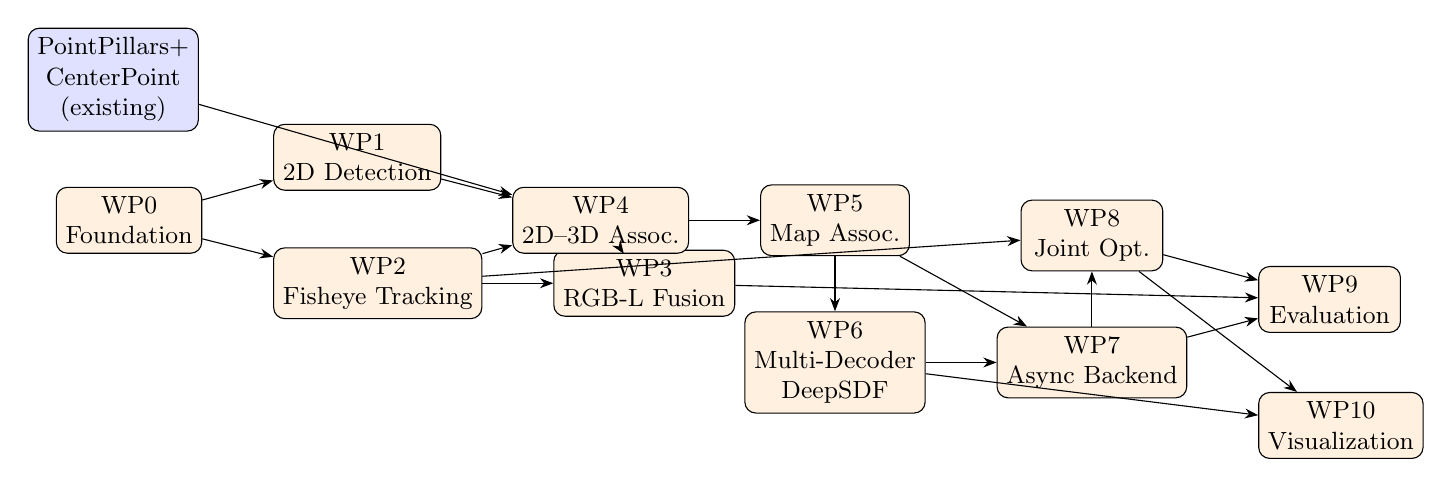
\begin{tikzpicture}[
  node distance=7mm and 9mm,
  wp/.style={rectangle, draw, rounded corners, align=center, minimum height=8mm, minimum width=18mm, font=\small, fill=orange!12},
  existing/.style={wp, fill=blue!12},
  >=Stealth
]
\node[wp] (wp0) {WP0\\Foundation};
\node[existing, above=of wp0, xshift=-2mm] (pp) {PointPillars+\\CenterPoint\\(existing)};

\node[wp, right=of wp0, yshift=8mm] (wp1) {WP1\\2D Detection};
\node[wp, right=of wp0, yshift=-8mm] (wp2) {WP2\\Fisheye Tracking};

\node[wp, right=of wp2] (wp3) {WP3\\RGB-L Fusion};
\node[wp, right=of wp1, yshift=-8mm] (wp4) {WP4\\2D--3D Assoc.};

\node[wp, right=of wp4] (wp5) {WP5\\Map Assoc.};
\node[wp, below=of wp5] (wp6) {WP6\\Multi-Decoder\\DeepSDF};
\node[wp, right=of wp6] (wp7) {WP7\\Async Backend};
\node[wp, above=of wp7] (wp8) {WP8\\Joint Opt.};
\node[wp, right=of wp7, yshift=8mm] (wp9) {WP9\\Evaluation};
\node[wp, right=of wp7, yshift=-8mm] (wp10) {WP10\\Visualization};

\draw[->] (wp0) -- (wp1);
\draw[->] (wp0) -- (wp2);
\draw[->] (pp) -- (wp4);
\draw[->] (wp2) -- (wp3);
\draw[->] (wp2) -- (wp4);
\draw[->] (wp3) -- (wp4);
\draw[->] (wp1) -- (wp4);
\draw[->] (wp4) -- (wp5);
\draw[->] (wp5) -- (wp6);
\draw[->] (wp5) -- (wp7);
\draw[->] (wp6) -- (wp7);
\draw[->] (wp2) -- (wp8);
\draw[->] (wp7) -- (wp8);
\draw[->] (wp3) -- (wp9);
\draw[->] (wp7) -- (wp9);
\draw[->] (wp8) -- (wp9);
\draw[->] (wp6) -- (wp10);
\draw[->] (wp8) -- (wp10);
\end{tikzpicture}%
}
\caption{Work-package dependency graph. WP0/WP1/WP2 can start in parallel; WP6 (DeepSDF decoder training) can also be trained offline in parallel with WP2--WP4 since it only needs class labels and ShapeNet assets, not a working SLAM front-end.}
\end{figure}

\noindent\textbf{Suggested milestones:}
\begin{enumerate}[nosep]
  \item \textbf{M1 --- Perception ready:} WP0, WP1, WP4 complete; class-labeled, associated 2D--3D detections available offline on recorded sequences (no tracking yet).
  \item \textbf{M2 --- Metric visual tracking ready:} WP2, WP3 complete; fisheye camera produces metric-scale trajectories comparable to Table~I.
  \item \textbf{M3 --- Static object mapping:} WP5, WP6 complete; single-threaded (synchronous) reconstruction produces class-correct meshes anchored in the map.
  \item \textbf{M4 --- Real-time system:} WP7, WP8 complete; asynchronous pipeline meets target FPS with bounded KF BA latency.
  \item \textbf{M5 --- Validated system:} WP9, WP10 complete; ATE and latency tables reproduced on KITTI/nuScenes/custom data.
\end{enumerate}

% ----------------------------------------------------------------------
\section{Architectural Decisions and Risks}
\label{sec:risks}

\begin{itemize}
  \item \textbf{Language boundary (C++ vs.\ Python).} ORB-SLAM3 is a C++ library; the current repository is pure Python/PyTorch. The original DSP-SLAM bridges this with pybind11 (C++ SLAM core, Python shape-optimization callbacks). Recommend following the same pattern rather than re-implementing a SLAM front-end in Python, to avoid re-deriving mature, well-tested tracking/BA code. This should be decided \emph{before} WP2 starts, since it determines the entire process/threading model.
  \item \textbf{True parallelism for the async back-end (WP7).} Algorithm~2 assumes worker threads run genuinely in parallel with the mapping thread. If the DeepSDF optimization runs in Python, CPython's GIL will serialize pure-Python work; heavy tensor ops release the GIL during PyTorch's C++/CUDA execution, which likely suffices, but this should be measured early (a small prototype benchmark) rather than assumed. A process pool (via \texttt{multiprocessing}) is the fallback if thread-based concurrency proves insufficient.
  \item \textbf{Class taxonomy mismatch.} \texttt{checkpoint\_nuscenes\_center.pth} (the CenterPoint head selected for this plan) is trained for \texttt{Car/Pedestrian/Cyclist}; the target taxonomy is \texttt{car/bus/motorcycle/pedestrian}. Retraining (or fine-tuning) the CenterPoint head, and sourcing/curating bus and motorcycle instances in the training data, is on the critical path for WP1 and should be scheduled early given training time.
  \item \textbf{CenterPoint-only inference path.} Choosing the CenterPoint head as the sole go-forward detector means the anchor head (\texttt{PointPillars}, \texttt{postprocess.py}, \texttt{anchor.py}, \texttt{nms.py}) becomes dead code for this project; it can stay in the repository for reference/comparison but should not be a dependency of any new WP. \texttt{DetectionPipeline} additionally needs the \texttt{use\_center} inference wiring called out in WP1 before it can load \texttt{checkpoint\_nuscenes\_center.pth} at all.
  \item \textbf{DeepSDF training data for non-standard classes.} ShapeNet has strong car coverage but weaker/no dedicated bus or motorcycle categories at the same fidelity; asset curation and canonical-orientation preprocessing for these classes is a real risk to reconstruction quality and should be scoped during WP6 planning, not discovered mid-implementation.
  \item \textbf{Licensing.} ORB-SLAM3 is GPLv3-licensed; any distribution of the integrated system inherits that obligation. Worth flagging now if the project has different distribution plans.
  \item \textbf{Sensor rig availability.} WP3 (fisheye + LiDAR metric fusion) needs real or simulated fisheye-LiDAR data with known extrinsics; if no such rig/dataset is available in-house yet, nuScenes (pinhole) can validate WP4--WP9 first, deferring true fisheye validation to whatever dataset is used to reproduce Table~I's fisheye rows (CBNU-style or custom).
  \item \textbf{Evaluation dataset gaps.} Table~I/II reproduction requires GT trajectories (GNSS/INS or dataset-provided poses); confirm which target datasets actually have usable ground truth before committing to WP9's exact metrics.
\end{itemize}

% ----------------------------------------------------------------------
\section{Proposed Repository Additions}

To keep the existing, working \texttt{lidar\_detection} package untouched as the Det3D component, new work is proposed as sibling top-level packages:

\small
\begin{verbatim}
Code_tensor/
|-- lidar_detection/     # existing, unchanged (Det3D)
|-- detection2d/         # WP1: YOLO11x-seg wrapper, class thresholds
|-- slam_frontend/       # WP2/3: ORB-SLAM3 bridge, RGB-L fusion, KB rectification
|-- association/         # WP4/5: 2D-3D matching, class-aware map association
|-- reconstruction/      # WP6: multi-decoder DeepSDF, pose/shape optimization
|   |-- decoders/        #   per-class pretrained DeepSDF weights
|-- async_backend/       # WP7: task/result queues, worker pool, placeholders
|-- evaluation_slam/     # WP9: ATE + latency benchmarking (SLAM-level;
|                        #   existing lidar_detection/evaluation is per-frame only)
|-- datasets/            # WP0: streaming KITTI/nuScenes/custom adapters + calibration
\end{verbatim}
\normalsize

This keeps the pretrained detector reusable as-is (imported by \texttt{association/} as the Det3D call), while isolating the large amount of new, cross-cutting SLAM infrastructure.

% ----------------------------------------------------------------------
\section{Summary}

The repository today implements roughly one of the thirteen components listed in Table~\ref{tab:gap} (3D detection, standardized on the CenterPoint head and \texttt{checkpoint\_nuscenes\_center.pth}), plus a partial second (streaming dataset support). The remaining work --- a fisheye-capable visual tracking front-end, LiDAR metric-depth fusion, multi-class 2D detection, the class-consistent global association algorithm, per-class DeepSDF reconstruction, the asynchronous back-end, and joint pose-graph optimization --- is substantial and mostly independent of the existing PointPillars/CenterPoint code, which plugs in cleanly at a single, well-defined point (Algorithm~1, line~2) once the small \texttt{DetectionPipeline} wiring change in WP1 is made. The work packages above are ordered so that perception (WP0/1/4), tracking (WP2/3), and offline shape-model training (WP6) can proceed in parallel, converging on the asynchronous, jointly-optimized system (WP7/8) that the evaluation harness (WP9) then validates against the paper's own metrics.

\bibliographystyle{plain}
\bibliography{plan_refs}

\end{document}
